%----------------------------------------------------------------------------------------
%	PACKAGES AND THEMES
%----------------------------------------------------------------------------------------

\PassOptionsToPackage{table}{xcolor}
\documentclass[aspectratio=169,xcolor=dvipsnames,svgnames,x11names,fleqn]{beamer}
% \documentclass[aspectratio=169,xcolor=dvipsnames,fleqn]{beamer}

\usetheme{RedVelvet}
\usefonttheme[onlymath]{serif}
\usepackage{xspace}
\usepackage{amsmath}
\usepackage{amssymb}
\usepackage{amsfonts}
\usepackage{color}
\usepackage{physics}
% \usepackage{mathbb}
\usepackage{rahul_math}
\usepackage{bigints}

  
\usepackage{graphicx} % Allows including images
\usepackage{booktabs} % Allows the use of \toprule, \midrule and \bottomrule in tables
\usepackage{tikz,pgfplots}
\usepackage{subfigure}
\usetikzlibrary{arrows}
\usepackage{minted}
\definecolor{LightGray}{gray}{0.9}
\definecolor{cream}{rgb}{0.92, 0.9, 0.55}
\definecolor{lightblue}{rgb}{0.68, 0.85, 0.9}


\usepackage{xcolor-material}
\usetikzlibrary{fit}
\tikzset{%
apple/.pic={
  \fill [MaterialBrown] (-1/8,0)  arc (180:120:1 and 3/2) coordinate [pos=3/5] (@)-- ++(1/6,-1/7)  arc (120:180:5/4 and 3/2) -- cycle;
  \fill [MaterialLightGreen500] (0,-9/10)  .. controls ++(180:1/8) and ++(  0:1/4) .. (-1/3,  -1) .. controls ++(180:1/3) and ++(270:1/2) .. (  -1,   0) .. controls ++( 90:1/3) and ++(180:1/3) .. (-1/2, 3/4) .. controls ++(  0:1/8) and ++(135:1/8) .. (   0, 4/7)
}
}

\newcommand{\leftdoublequote}{\textcolor{blue}{\scalebox{3}{``}}}

\newcommand{\rightdoublequote}{\textcolor{blue}{\scalebox{3}{''}}}


\usepackage{textcomp}
\usepackage{fontawesome}

\usepackage{overpic}

%----------------------------------------------------------------------------------------
%	TITLE PAGE
%----------------------------------------------------------------------------------------

\usepackage{tikz-qtree,tikz-qtree-compat}
\usetikzlibrary{calc}


\title[CPE 381: Signals and Systems]{CPE 381: Fundamentals of Signals and Systems for Computer Engineers} % The short title appears at the bottom of every slide, the full title is only on the title page
\subtitle{03 Continuous-Time Signals}

\author[Rahul Bhadani] {{\Large \textbf{Rahul Bhadani}}}

\institute[UAH] % Your institution as it will appear on the bottom of every slide, maybe shorthand to save space
{
    Electrical \& Computer Engineering,  The University of Alabama in Huntsville
}
\date

% \titlegraphic{
%    \includegraphics[width=0.4\linewidth]{figures/UAH_primary.png}
% }

\usepackage{hyperref}

  
  \urlstyle{same}
  
\begin{document}

%-------------------------------------------------
\begin{frame}
  \titlepage
\end{frame}

\begin{frame}{Announcement}
\begin{itemize}
    \item Homework 01 Due September 01 11:59 PM
    \item Quiz 01, based on Chapter 01 Continuous-Time Signals from the Textbook. Available from September 05, 12:01 AM to September 07, 11:59 PM. 30 Questions, 45 Minutes.
    \item Office hour: 08/28 Aug Wednesday, 1 PM - 3:30 PM. 
    \item No class on September 02, 2024: Labor Day, University Closed.
\end{itemize}
    
\end{frame}
%-------------------------------------------------
\begin{frame}{Outline}
   \tableofcontents
\end{frame}

%%%%%%%%%%%%%%%%%%%%%%%%%%%%%%%%%%%%%%%%%%%%%%%%%%%%%
\section{Motivation}

%-----------------------------------------

\begin{frame}{}
    \begin{center}
    \Huge \bf \color{DarkBlue}
    \faFire
    
    Motivation
\end{center}
\end{frame}


\begin{frame}{}
    \begin{center}
    \Huge \bf 
    
    Signals and Systems is `Grandfather' of Data Science for Electrical and Computer Engineers

\end{center}
\end{frame}

\begin{frame}{Classification of Signals}

We care about the following properties when dealing with signals:

\begin{itemize}
    \item Predictability:  Random or Deterministic
    \item Variations of time and amplitude: continuous, discrete (time or x-axis) / quantized (amplitude or y-axis)
    \item Periodic/Aperiodic
    \item Finite energy/finite power;  Infinite energy/Infinite power

\end{itemize}

\end{frame}

%%%%%%%%%%%%%%%%%%%%%%%%%%%%%%%%%%%%%%%%%%%%%%%%%%%%%
\section{Operation on Signals}

%-----------------------------------------

\begin{frame}{}
    \begin{center}
    \Huge \bf \color{DarkBlue}
    \faAreaChart
    
    Operation on Signals
\end{center}
\end{frame}

\begin{frame}{Basic Mathematical Operations}
\begin{itemize}
    \item Addition: $x(t) + y(t)$
\item Subtraction: $x(t) - y(t)$
\item Constant multiplication: $kx(t)$ where $k$ is a constant
\end{itemize}
\end{frame}

\begin{frame}{Time-shift}

\begin{itemize}
    \item $x(t - \tau) \to $ Signal is delayed
\item $x(t + \tau) \to $ Signal is advanced
\end{itemize}
  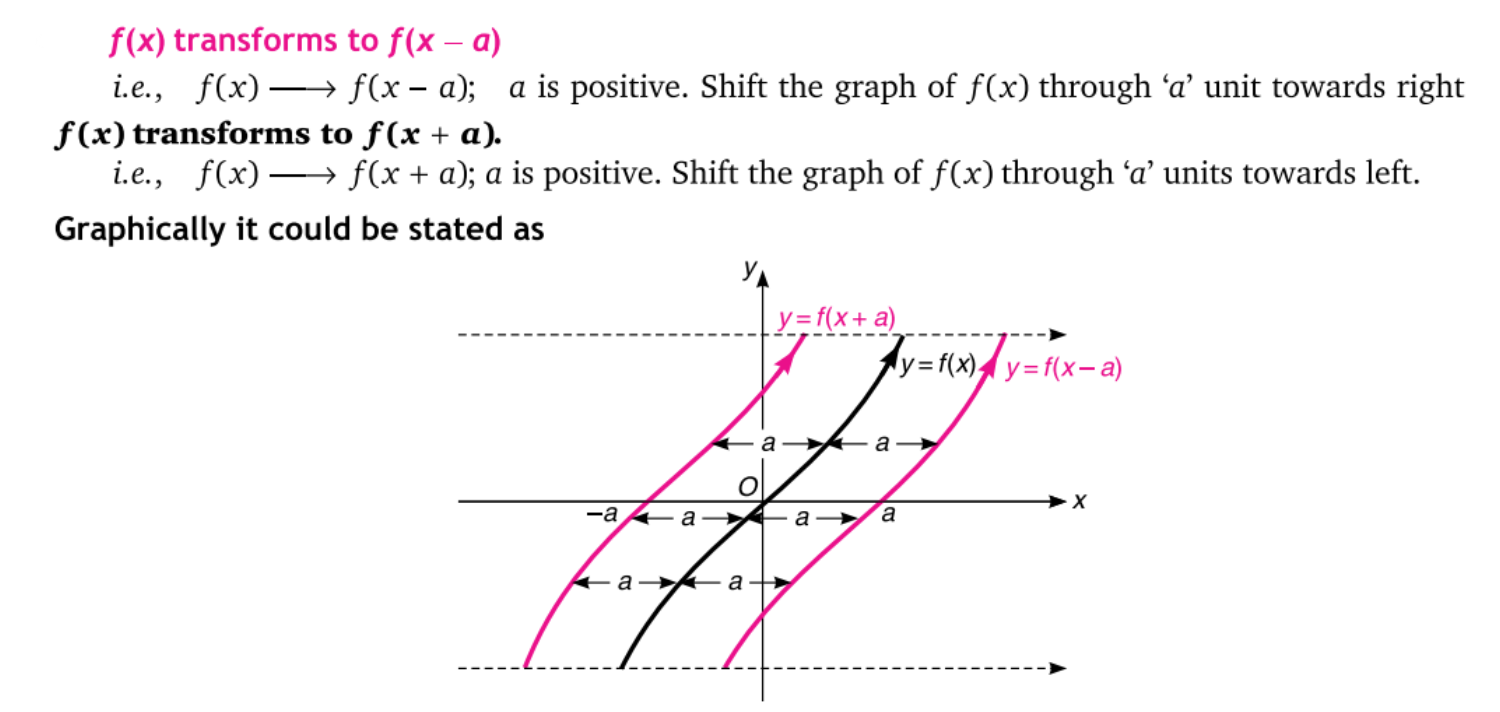
\includegraphics[width=0.8\linewidth,trim=0 0 0 0cm,clip]{figures/Signal_Delay.png}
    
\end{frame}

\begin{frame}{Time Reflection}
\begin{columns}
    \column{0.3\linewidth}
    \begin{itemize}
    \item $x(t) \to x(-t)$ : take  mirror image\textbf{ along the y-axis}
    \end{itemize}
      \column{0.7\linewidth}
      Note: The book doesn’t specify whether to take the mirror image along the y-axis or not and it is confusing because the signal used in example 1.3.1 is symmetric with respect to both the x and y axes.
       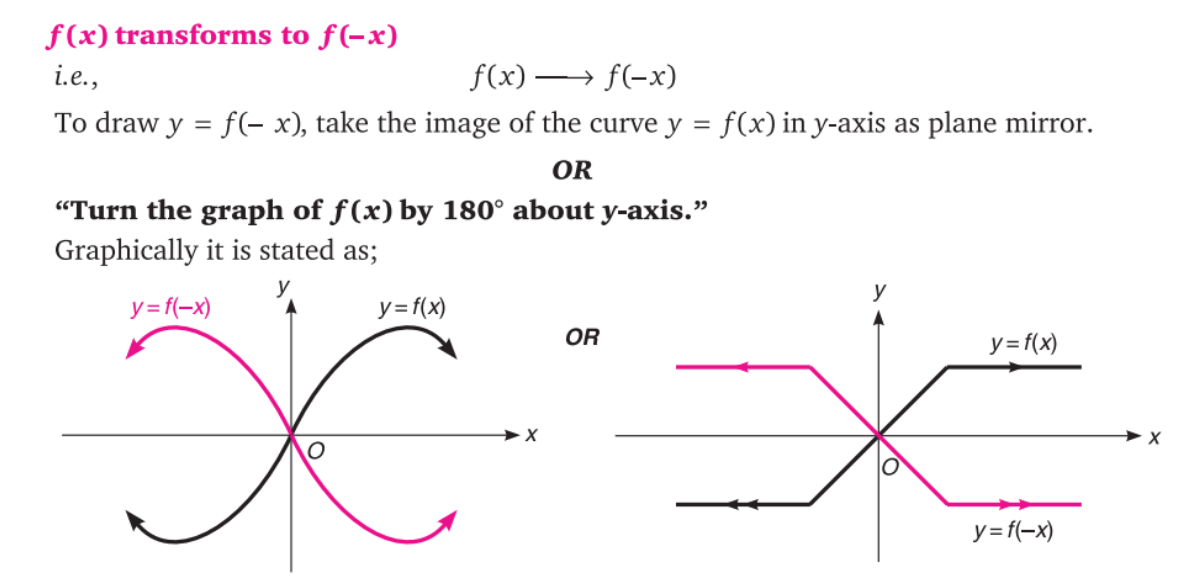
\includegraphics[width=0.9\linewidth,trim=0 0 0 0cm,clip]{figures/Time_Reflection.png}
\end{columns}
\end{frame}


\begin{frame}{Signal Stretching along $y$-axis}

    \begin{itemize}
    \item $f(x) \to a f(x); \quad a > 1$ : Stretch the graph of $f(x)$ `$a$' times along y-axis.
    \item $f(x) \to \cfrac{1}{a} f(x); \quad a > 1$ : Shrink the graph of $f(x)$ `$a$' times along y-axis.
    
    \end{itemize}

       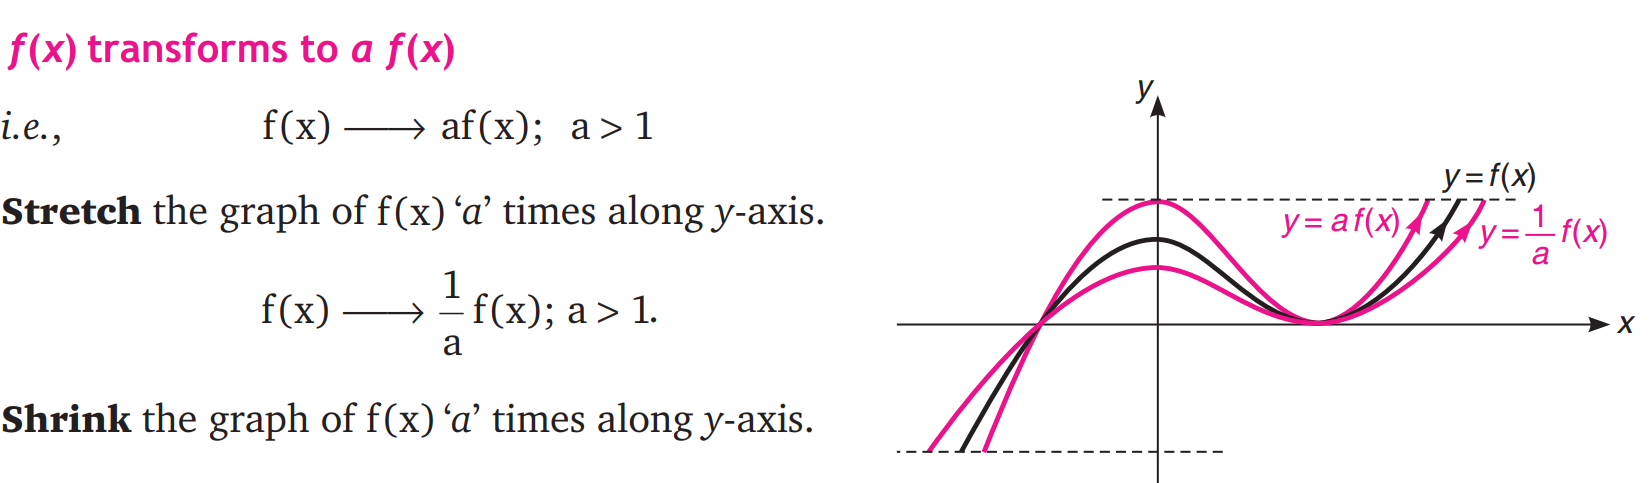
\includegraphics[width=0.9\linewidth,trim=0 0 0 0cm,clip]{figures/Signal_Stretch.png}

\end{frame}

\begin{frame}{Signal Stretching along $x$-axis}

    \begin{itemize}
    \item $f(x) \to a f(ax); \quad a > 1$ : Stretch the graph of $f(x)$ `$a$' times along x-axis.
    \item $f(x) \to f\bigg(\cfrac{1}{a} x\bigg); \quad a > 1$ : Shrink the graph of $f(x)$ `$a$' times along x-axis.
    
    \end{itemize}

       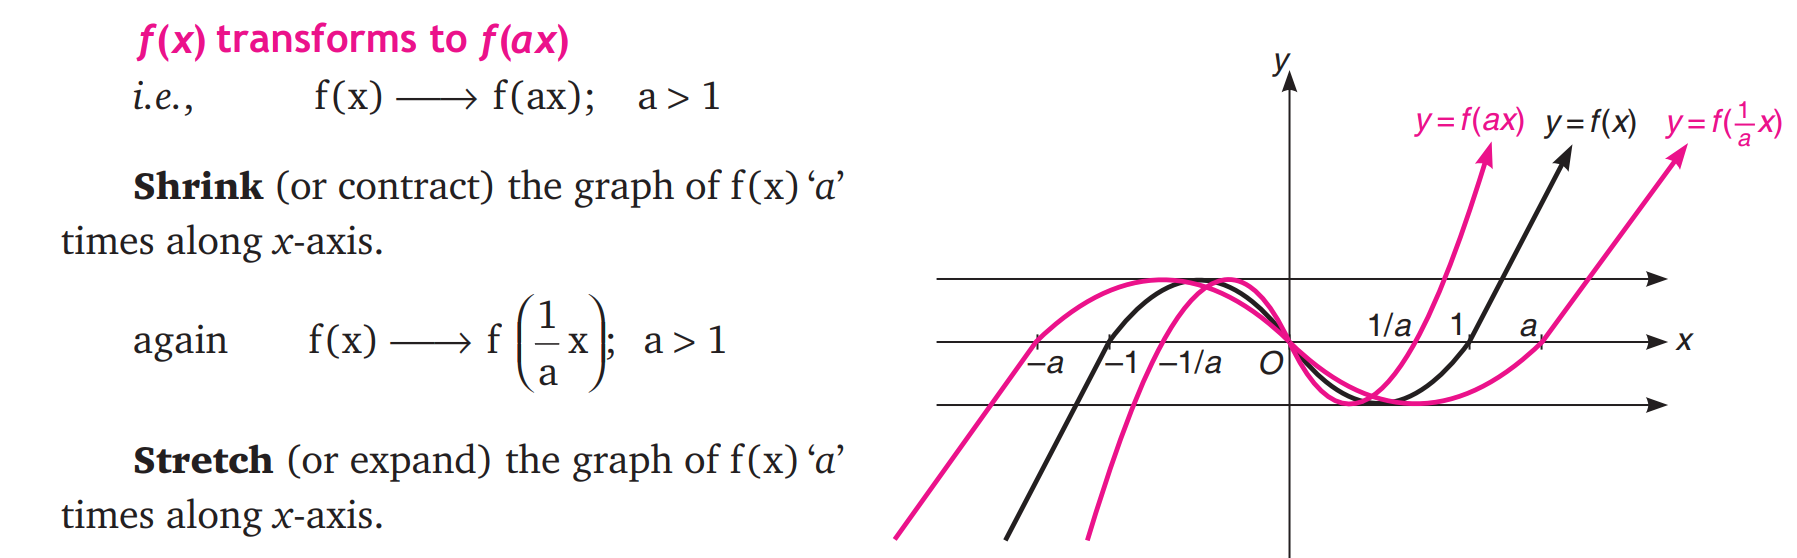
\includegraphics[width=0.9\linewidth,trim=0 0 0 0cm,clip]{figures/Signal_Sretch2.png}

\end{frame}

\begin{frame}{Example and MATLAB Code}


\begin{columns}
    \column{0.25\linewidth}
    $$
x(t) = 6t^2 + 4t + 70
$$
Code: \url{https://github.com/rahulbhadani/CPE381_FA25/blob/main/Code/signal_operation.m}

      \column{0.75\linewidth}
        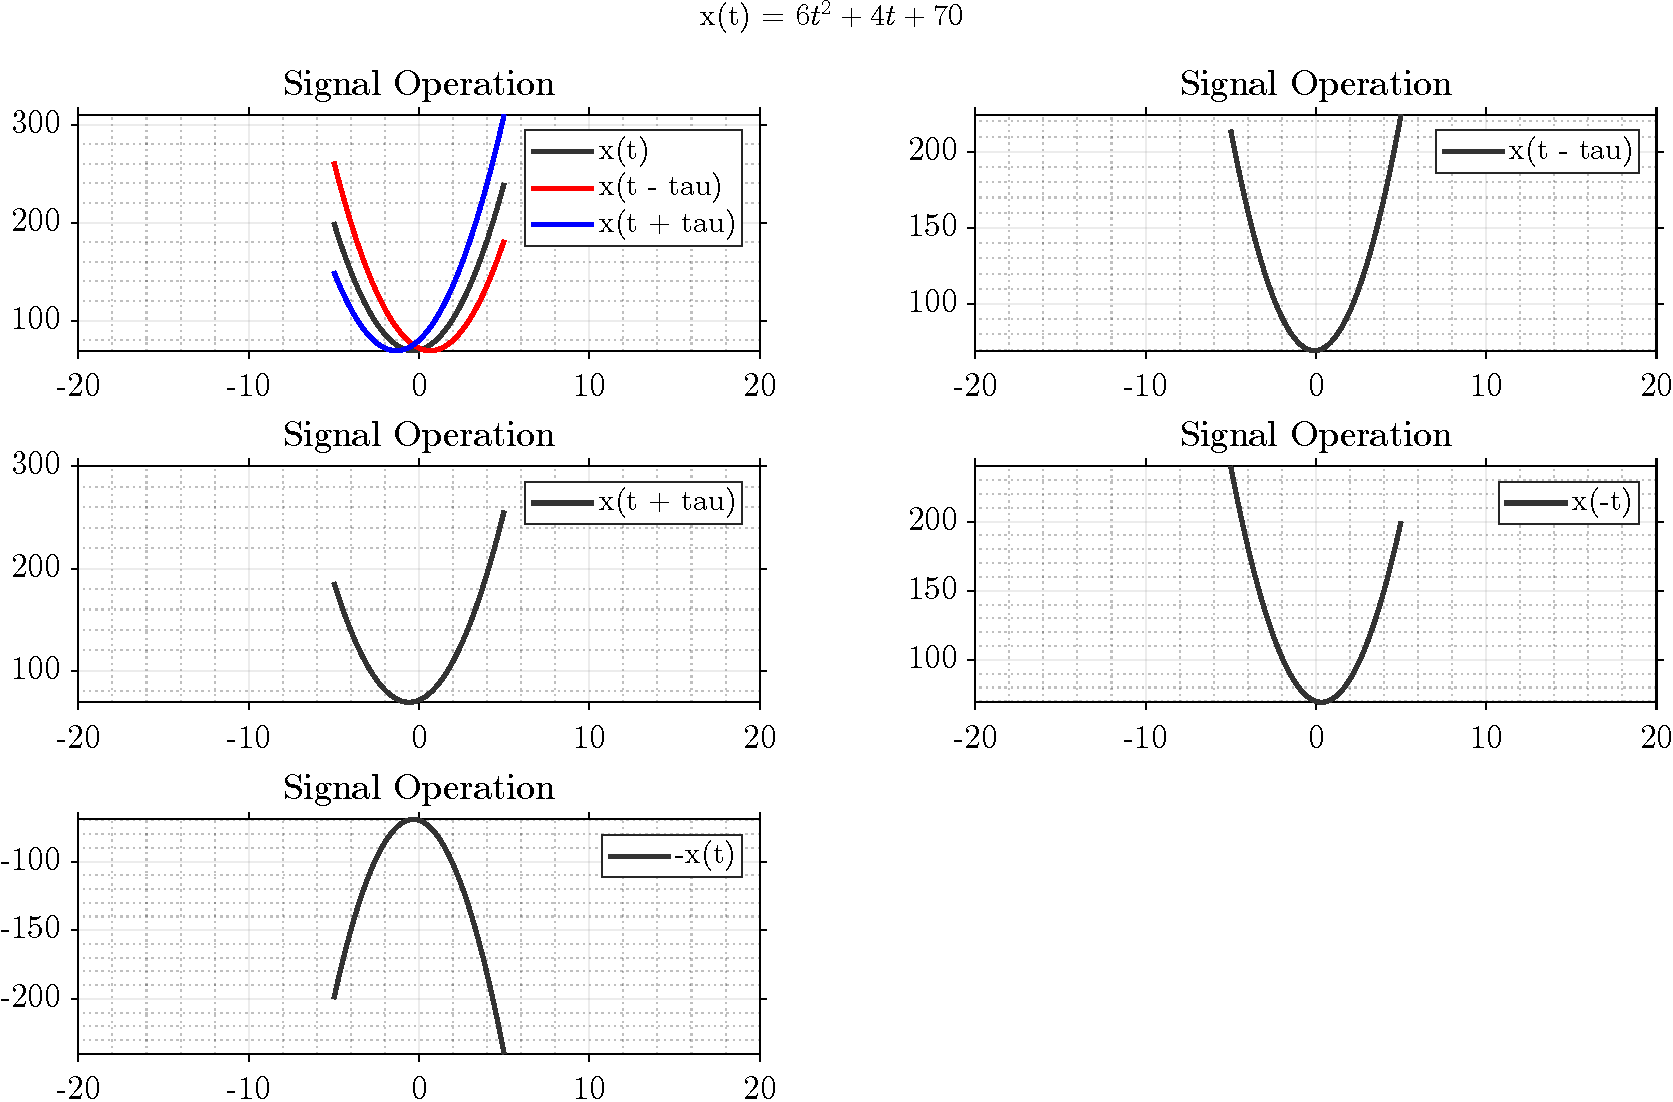
\includegraphics[width=0.99\linewidth,trim=0 0.0 0 1.0cm,clip]{figures/signal_operations.pdf}

\end{columns}
    
\end{frame}

\begin{frame}{Even and Odd Signals}
\begin{itemize}
    \item Even Signal: $x(t) = x(-t)$
\item Odd Signal:
$x(t) = -x(-t)$
\item Any signal can be represented by the sum of even and odd signals

$y(t) = y_e(t) + y_o(t)$

$$
y_e(t) = 0.5[ y(t)  + y(-t) ]$$

$$
y_o(t) = 0.5[y(t) - y(-t) ]
$$

\end{itemize}
\end{frame}

\begin{frame}{Periodic Signals}


\begin{itemize}
    \item Defined for all possible values of $t, -\infty < t < \infty$.
    \item 
There is the real value $T_0 \in \Rbb^+$, called the fundamental frequency such that $x(  t + kT_0 ) = x(t), k \in \Ibb$.

\item A constant signal is periodic of a non-definable fundamental period.
\item A $\cos(\omega t + \theta)$, $\omega = 2\pi/T_0$ ,
$\omega = 2, \theta = -\pi/2, A= 2$.

\vspace{5pt}

\bf \color{red}
What’s the fundamental frequency, $1/T_0$?
\end{itemize}
\end{frame}

\begin{frame}{Energy and Power of Signals}

{
\bf\color{red}What's the instantaneous power of a resistor?
}

    \begin{itemize}
        \item \textbf{Energy:}
        $$
        E_x = \int_{-\infty}^\infty | x(t)| ^2 dt
        $$

        \item \textbf{Power:}
        $$
        P_x = \lim_{T\to\infty}\cfrac{1}{2T} \int_{-T}^T | x(t)| ^2 dt
        $$
    \end{itemize}

    \bf A signal is called finite power if the signal power is finite.
\end{frame}


%%%%%%%%%%%%%%%%%%%%%%%%%%%%%%%%%%%%%%%%%%%%%%%%%%%%%
\section{Basic Signals as Building Blocks
}

%-----------------------------------------

\begin{frame}{}
    \begin{center}
    \Huge \bf \color{DarkBlue}
    \faBuilding
    
    Basic Signals as Building Blocks

\end{center}
\end{frame}

\begin{frame}{Complex Exponentials}
Consider $A = |A|e^{j\theta}$, $a = r + k\Omega_0$
\begin{itemize}
    \item $x(t) = Ae^{at}$ = ...
    \item Real part $f(t) = \Re{x(t)}, = ... $
    
    \vspace{20pt}
    
    $\quad  -|A|e^{rt} \leq f(t)) \geq |A|e^{rt}$. $r< 0$, $f(t)$ is damped, $r>0 $, $f(t)$ grows.
    \item  Imaginary part $g(t) = \Im{x(t)}, = ... $
    
    \vspace{20pt}
\end{itemize}
    
\end{frame}

\begin{frame}{Sinusoids}
A sinusoid of the general form:
$$
A\cos(\Omega_0 t + \theta) = A\sin (\Omega_0 t + \theta + \pi/ 2), \quad -\infty < t < \infty
$$

\begin{itemize}
    \item $A$ is the amplitude
    \item $\Omega_0 = 2\pi f_0$ is angular frequency in \texttt{rad/s}.
    \item $\theta$ is phase shift
    \item Fundamental period $T_0$ is 

    $$
    T_0 = \cfrac{2\pi}{\Omega_0} = \cfrac{1}{f_0}
    $$
\end{itemize}
    
\end{frame}

\begin{frame}{Rectangular pulse and Unit impulse}

\begin{columns}
    \column{0.7\linewidth}
    \begin{itemize}
        \item  A rectangular pulse of duration $\Delta$ and unit area:
        \begin{equation*}
            \begin{aligned}
                p_\Delta(t)= \begin{cases}
                    \cfrac{1}{\Delta},\quad -\Delta/2 \leq t \leq \Delta/2\\
                    0, \quad \textrm{otherwise}
                \end{cases}
            \end{aligned}
        \end{equation*}
        \item Unit Impulse:
        \begin{equation*}
            \delta(t) = \lim_{\Delta \to 0}p_\Delta (t)
        \end{equation*}
        \item \bf \color{red} Calculate 
        $$
        \int_{ -\infty}^{t}   p_\Delta(t) 
        $$
        Hint: there are three possible cases.
    \end{itemize}
    \column{0.3\linewidth}
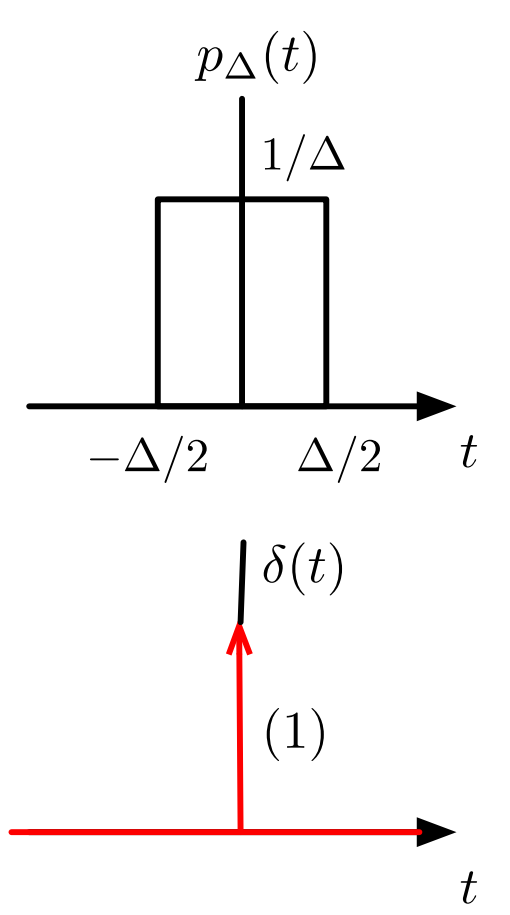
\includegraphics[width=0.7\linewidth,trim=0 0 0 0cm,clip]{figures/unitpulse.png}
\end{columns}
\end{frame}

\begin{frame}{Unit Step}

    \small
\begin{columns}
    \column{0.6\linewidth}
    \begin{itemize}
        \item  Integration of rectangular pulse:
        \begin{equation*}
            \begin{aligned}
                u_\Delta(t)= \int_{ -\infty}^{t}   p_\Delta(t) = \begin{cases}
                    1,\quad t \geq \cfrac{\Delta}{2}\\
                    \tfrac{1}{\Delta}(t + \tfrac{\Delta}{2}), \quad \cfrac{\Delta}{2} \leq t \leq \cfrac{\Delta}{2}\\
                    0, \quad t < -\cfrac{\Delta}{2}
                \end{cases}
            \end{aligned}
        \end{equation*}
        \item Limit case:
        \begin{equation*}
           \lim_{\Delta \to 0}u_\Delta (t) = \begin{cases}
                    1,\quad t \geq 0\\
                    0, \quad t <0
                \end{cases}
        \end{equation*}
      
    \end{itemize}
    \column{0.4\linewidth}
    \begin{itemize}
          \item A common case is to ignore $t=0$ case, which gives us unit step function as
        \begin{equation*}
        u(t) = \begin{cases}
                    1,\quad t \geq 0\\
                    0, \quad t <0
                \end{cases}
        \end{equation*}
    \end{itemize}
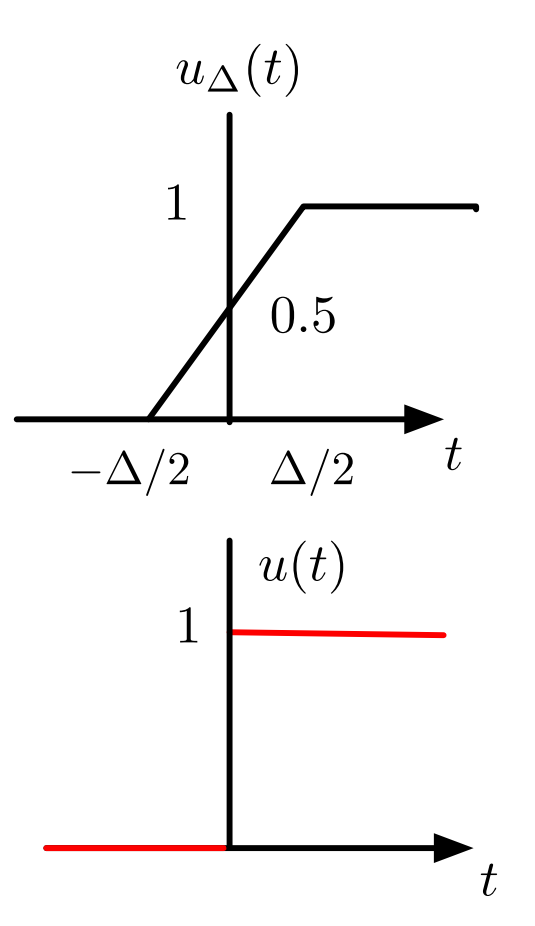
\includegraphics[width=0.35\linewidth,trim=0 0 0 0cm,clip]{figures/unitstep.png}
\end{columns}
\end{frame}

\begin{frame}{Ramp Signal}
The ramp signal is $r(t) = t u(t)$
\begin{columns}
 \column{0.4\linewidth}
    \begin{itemize}
        \item The relation between the ramp, the unit step, and the unit impulse:
        \begin{equation*}
            \begin{aligned}
                \cfrac{dr(t)}{dt} & = u(t)\\
                \cfrac{d^2r(t)}{dt^2} & = \delta(t)
            \end{aligned}
        \end{equation*}
    \end{itemize}
     \column{0.6\linewidth}
     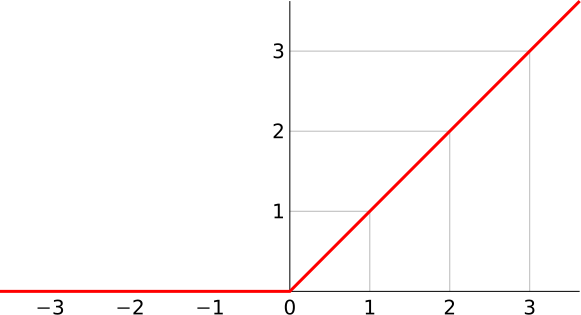
\includegraphics[width=0.65\linewidth,trim=0 0 0 0cm,clip]{figures/ramp_function.png}
    \end{columns}
\end{frame}

\begin{frame}{Triangular Pulse}
The triangular pulse is 
\begin{columns}
 \column{0.4\linewidth}
 \begin{equation*}
    \begin{aligned}
        \Lambda(t) = \begin{cases}
            t ,\quad 0 \leq t \leq 1\\
            -t + 2, \quad 1 < t \leq 2\\
            0,\quad \textrm{otherwise}
        \end{cases}
    \end{aligned}
\end{equation*}
    \begin{itemize}
        \item $ \Lambda(t)$ can also be written as:
        \begin{equation*}
            \begin{aligned}
              \Lambda(t) =   r(t) - 2r(t-1) + r(t-2)
            \end{aligned}
        \end{equation*}
    \end{itemize}
     \column{0.6\linewidth}
     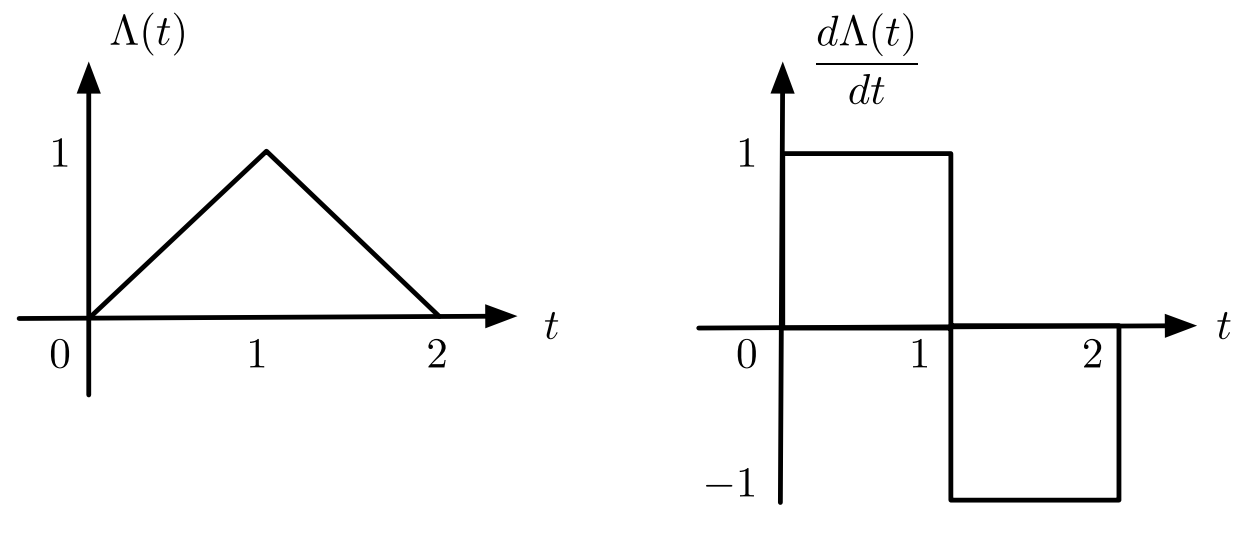
\includegraphics[width=0.85\linewidth,trim=0 0 0 0cm,clip]{figures/triangular_pulse.png}
    \end{columns}
\end{frame}

\begin{frame}[allowframebreaks]{Triangular Pulse as Ramp Functions}
Let's verify this by evaluating \( \Lambda(t) \) at different intervals:

\begin{columns}
    \column{0.5\linewidth}
     First, find out the first part:

    \begin{equation*}
            \begin{aligned}
              \Lambda_1(t) =  \begin{cases}
            t ,\quad 0 \leq t \leq 1\\
            0,\quad \textrm{otherwise}
        \end{cases}
            \end{aligned}
        \end{equation*}
    which can be written as:

can be written using the ramp function \( r(t) \) as:
    \begin{equation*}
        \Lambda_1(t) = r(t) - r(t-1)
    \end{equation*}
    \column{0.5\linewidth}
    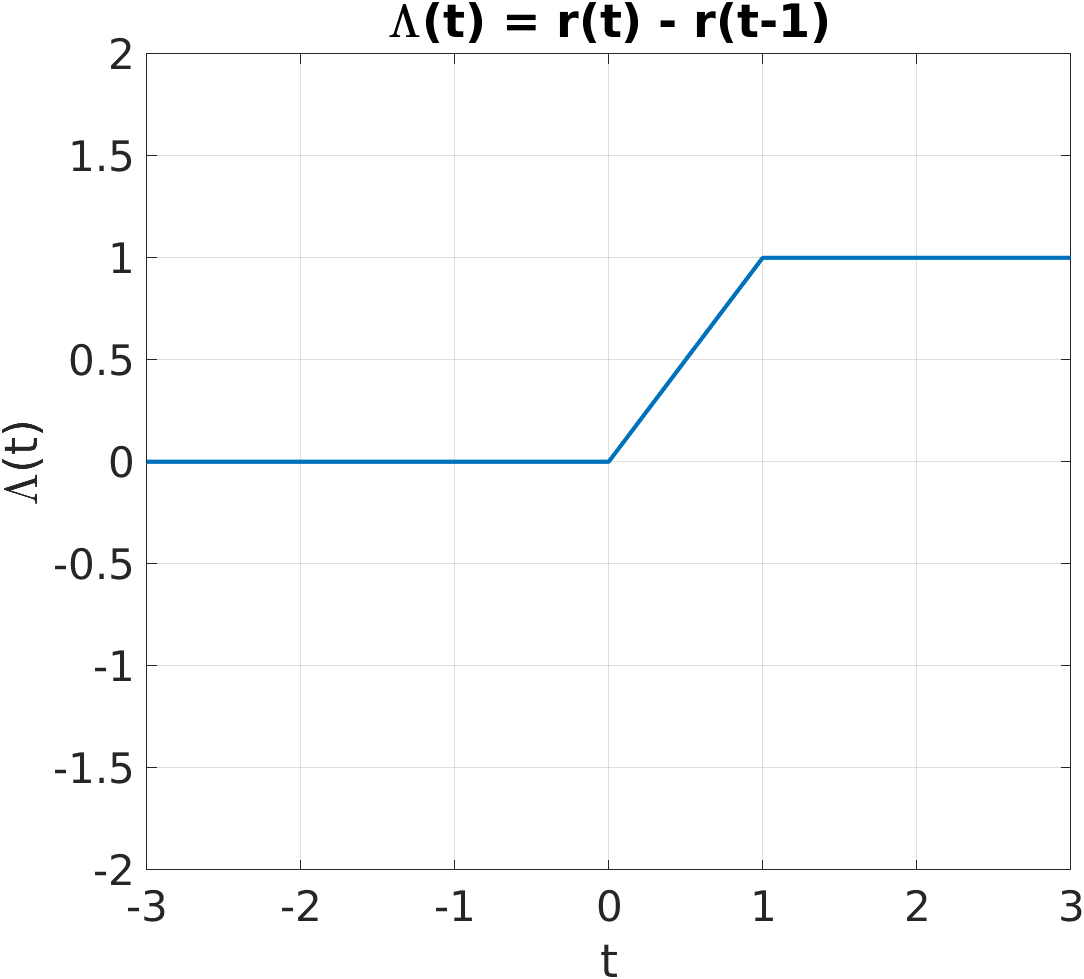
\includegraphics[width=0.75\linewidth,trim=0 0 0 0cm,clip]{figures/lambda_1.png}
\end{columns}

\begin{columns}
    \column{0.5\linewidth}
    Second part:
     \begin{equation*}
            \begin{aligned}
              \Lambda_1(t) =  \begin{cases}
            -t + 2, \quad 1 < t \leq 2\\
            0,\quad \textrm{otherwise}
        \end{cases}
            \end{aligned}
        \end{equation*}

 which can be written as:

can be written using the ramp function \( r(t) \) as:
    \begin{equation*}
        \Lambda_1(t) = r(t-2) - r(t-1)
    \end{equation*}
    \column{0.5\linewidth}
    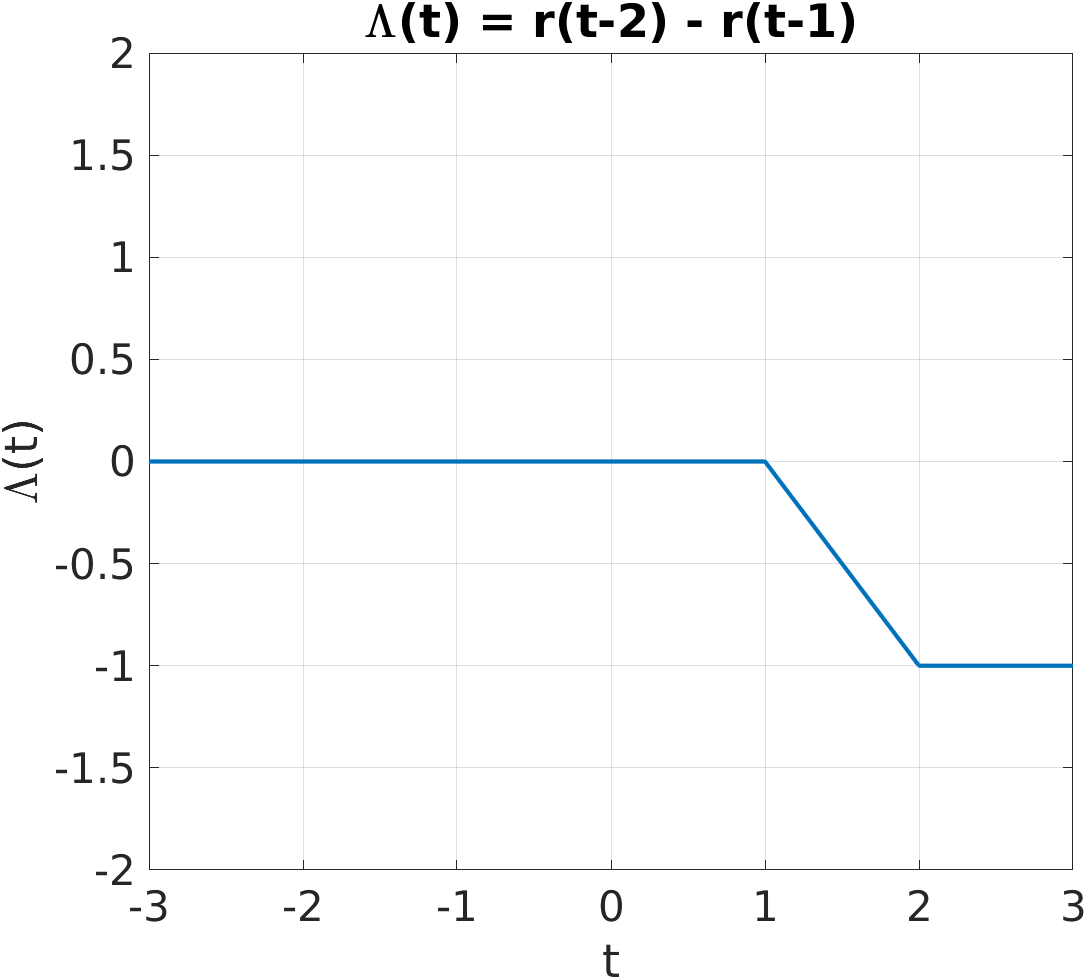
\includegraphics[width=0.95\linewidth,trim=0 0 0 0cm,clip]{figures/lambda_2.png}
\end{columns}

   Putting together 
  
   \centering
   
     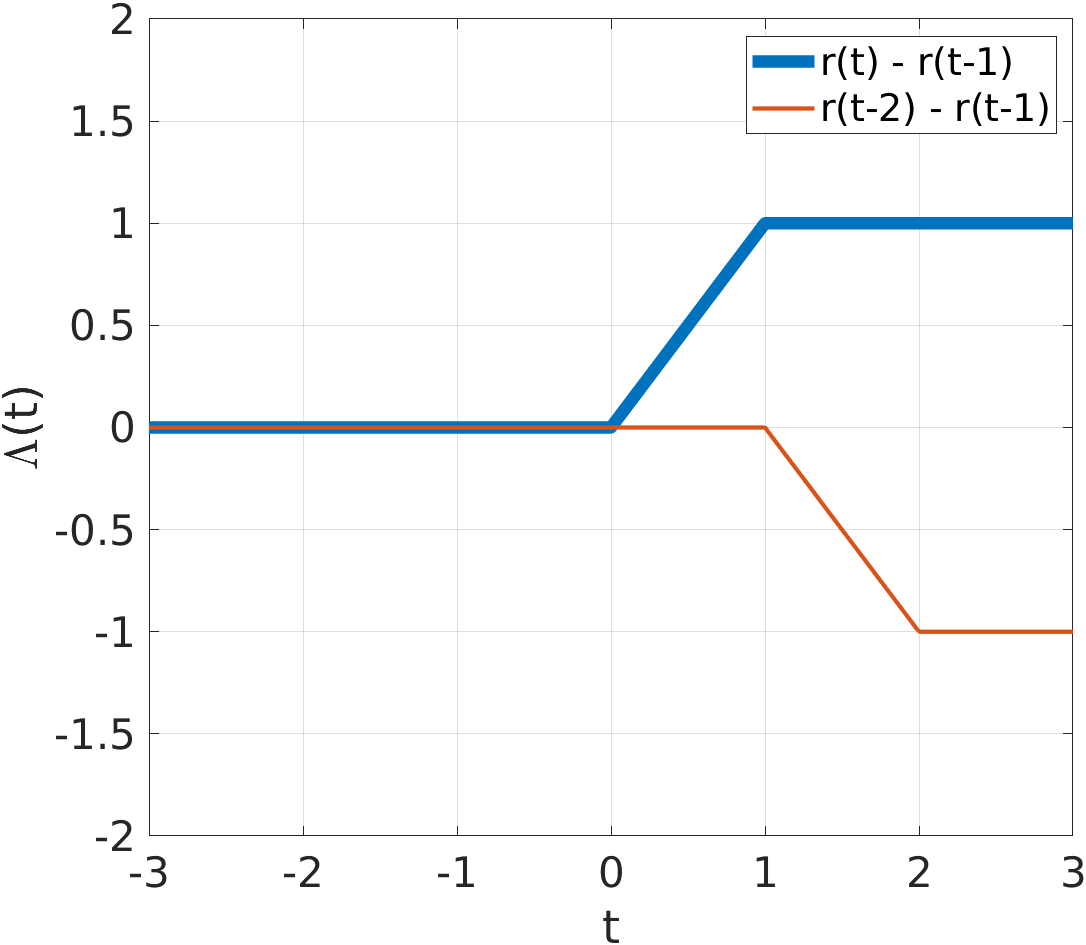
\includegraphics[width=0.40\linewidth,trim=0 0 0 0cm,clip]{figures/lambda_1_2.png}

\end{frame}

\begin{frame}{Sifting Property}
The product of $f (t)$ and $\delta(t)$ gives zero everywhere except at the origin where we get an impulse of area $f (0)$, that is, $f (t)\delta(t) = f (0)\delta(t)$.

Hence,

$$
\int_{-\infty}^\infty f(t)\delta(t)dt = \int_{-\infty}^\infty f(0)\delta dt = f(0) \int_{-\infty}^\infty\delta (t) dt  = f(0)
$$
This is called \textbf{Sifting Property}.

If we delay or advance the $\delta(t)$ function in the integrated, the result is that all values of $f (t)$ are sifted out except for the value corresponding to the location of the delta function, that is,

$$
\int_{-\infty}^\infty f(t)\delta(t - \tau)dt  = \int_{-\infty}^\infty f(\tau)\delta(t- \tau) dt  = f(\tau) \int_{-\infty}^\infty \delta(t-\tau) dt  = f(\tau)\quad \text{for any }\tau
$$

\end{frame}

\begin{frame}{Generic Representation of Signals}
Hence, if we do integration in terms of variable $\tau$, we get a generic representation of signals in terms of impulse and shifted impulse.
\begin{columns}
    \column{0.45\linewidth}
   $x(t) = \int_{-\infty}^\infty x(\tau ) \delta(t-\tau)d\tau $

     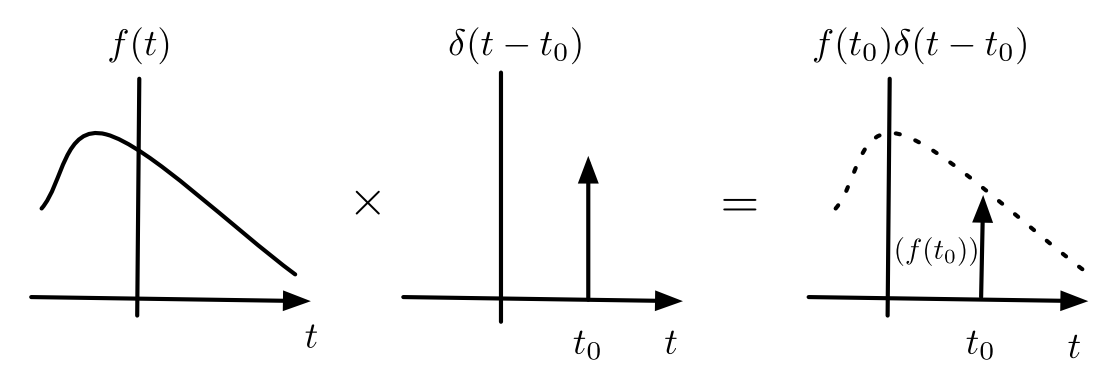
\includegraphics[width=0.85\linewidth,trim=0 0 0 0cm,clip]{figures/signal_multiplication.png}

     \column{0.55\linewidth}
      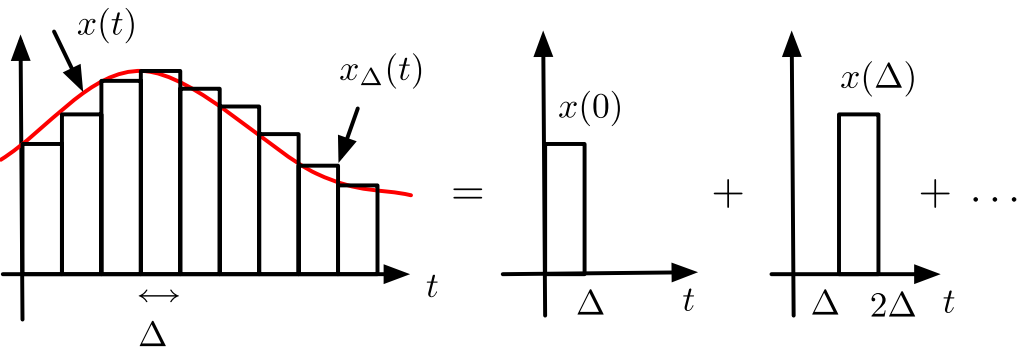
\includegraphics[width=0.85\linewidth,trim=0 0 0 0cm,clip]{figures/signal_sums.png}
      \begin{itemize}
          \item Approximation of $x(t)$:
          \footnotesize
          {
          \begin{equation*}
              x_\Delta(t) = \sum_{-\infty}^\infty x_\Delta(t-k\Delta) = \sum_{-\infty}^\infty x(k\Delta) p_\Delta(t-k\Delta)\Delta
          \end{equation*}
          }
      \end{itemize}
\end{columns}
In the limit as $\Delta \to 0$ these pulses become impulses, separated by an infinitesimal value:

$\lim_{\Delta \to 0 }x_\Delta(t) \to x(t)  =  \int_{-\infty}^\infty x(\tau ) \delta(t-\tau)d\tau $
    
\end{frame}

%%%%%%%%%%%%%%%%%%%%%%%%%%%%%%%%%%%%%%%%%%%%%%%%%%%%%
\section{Modulation and Windowing}

%-----------------------------------------

\begin{frame}{}
    \begin{center}
    \Huge \bf \color{DarkBlue}
    \faLineChart
    
    Modulation and Windowing

\end{center}
\end{frame}

\begin{frame}{Modulation}
    Multiplication by a complex exponential shifts the frequency of the original signal.
    \begin{block}{Definition}
        Superimposing a low-frequency signal on a high-frequency carrier signal is called \textbf{Modulation}.
    \end{block}
    
   \textbf{Example:}

   Consider an exponential signal $x(t) = e^{j\Omega_0 t}$ of frequency $\Omega_0$. If we multiply an exponential $e^{j\phi t}$ with $x(t)$, then:
   $$
   x(t)e^{j\phi t} = e^{j(\Omega_0 + \phi) t} = \cos((\Omega_0 + \phi) t) + j \sin((\Omega_0 + \phi) t)
   $$

    $
    \phi > 0: 
    $ the frequency of new exponential is greater than $\Omega_0$, otherwise lower.
   
    
\end{frame}

\begin{frame}{Various Types of Modulation}
$A(t)cos( \Omega(t)t + \theta(t) )$
    \begin{itemize}
        \item $A(t)$ changes: Amplitude Modulation
\item $\Omega(t)$ changes: Frequency Modulation
\item $\theta(t)$ changes: Phase Modulation
    \end{itemize}
\end{frame}

\begin{frame}{Windowing}
   
\begin{columns}
    \column{0.5\linewidth}
     For a window signal $w(t)$, the time-windowed signal 
     
     $x(t)w(t)$ displays $x(t)$ within the support of $w(t)$.
     
 \textbf{Example:}

    $x(t) = \sin(2\pi t)$

    \begin{equation*}
        w(t) = \begin{cases} 1 \quad \text{if } -0.5 \leq t \leq 0.5 \\ 0 \quad \text{otherwise} \end{cases}
    \end{equation*}

\small

    Code for the graph: \url{https://github.com/rahulbhadani/CPE381_FA25/blob/main/Code/windowing.m}
    \column{0.5\linewidth}
         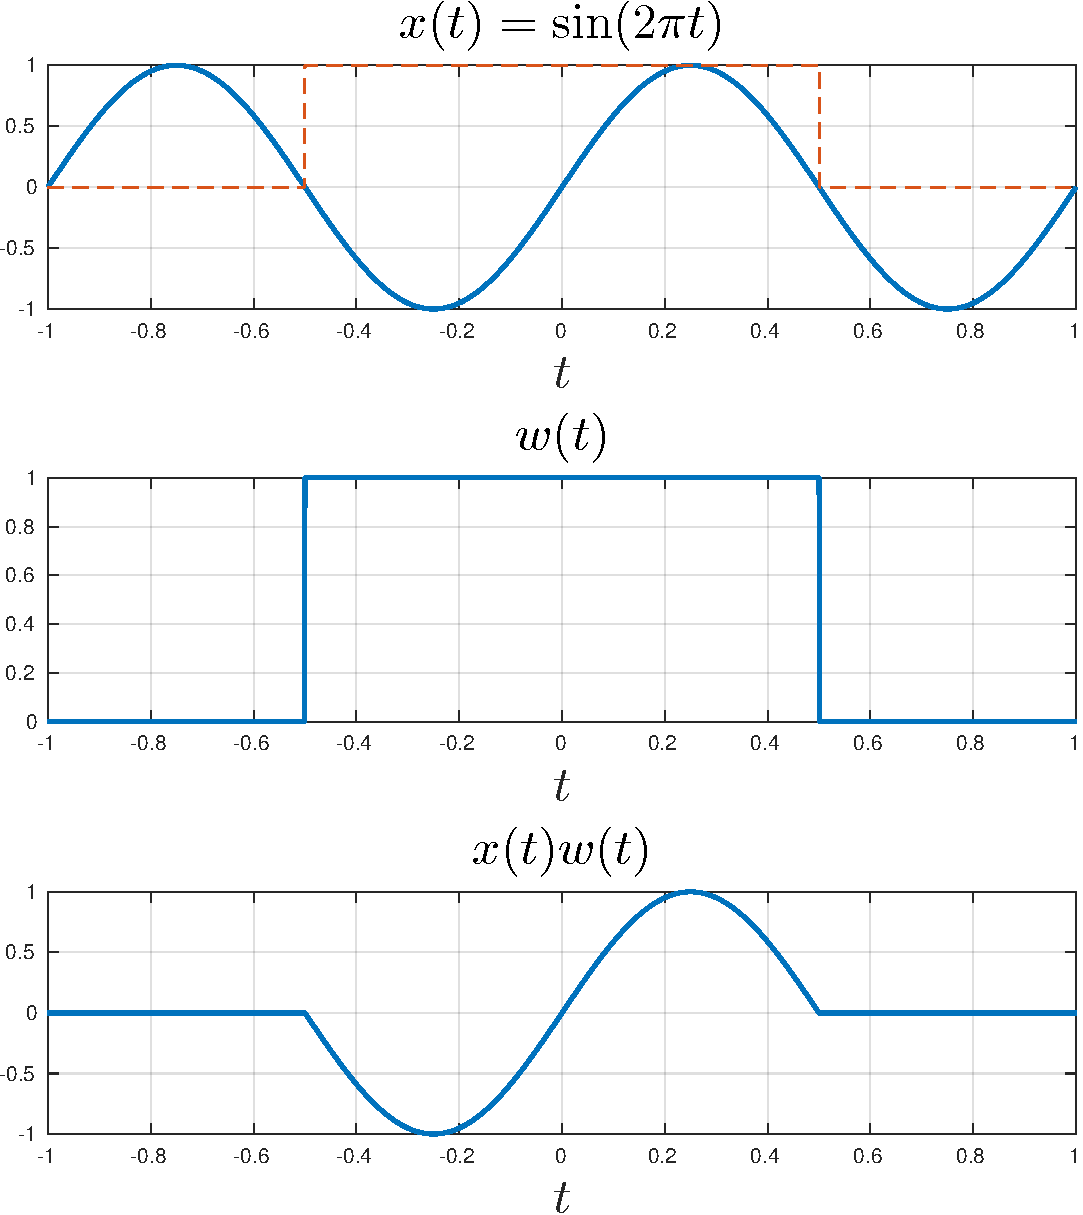
\includegraphics[width=0.65\linewidth,trim=0 0 0 0cm,clip]{figures/signal_windowing.pdf}
\end{columns}
   
\end{frame}

\begin{frame}{Classwork}
    
\end{frame}

\begin{frame}{Classwork}
    
\end{frame}
\begin{frame}{Classwork}
    
\end{frame}
\begin{frame}{Classwork}
    
\end{frame}
\begin{frame}{Classwork}
    
\end{frame}
\begin{frame}{Classwork}
    
\end{frame}
\begin{frame}{Classwork}
    
\end{frame}
\begin{frame}{Classwork}
    
\end{frame}
\begin{frame}{Classwork}
    
\end{frame}

\begin{frame}{Up Next}
\begin{itemize}
    \item Continuous-time Systems
    \begin{itemize}
        \item Linear-Time Invariance
        \item Static vs Dynamic Systems
        \item Convolutional Integral
        \item BIBO Stability
    \end{itemize}
\end{itemize}
    
\end{frame}
\end{document}